\documentclass[10pt]{article}\usepackage[]{graphicx}\usepackage[]{xcolor}
% maxwidth is the original width if it is less than linewidth
% otherwise use linewidth (to make sure the graphics do not exceed the margin)
\makeatletter
\def\maxwidth{ %
  \ifdim\Gin@nat@width>\linewidth
    \linewidth
  \else
    \Gin@nat@width
  \fi
}
\makeatother

\definecolor{fgcolor}{rgb}{0.345, 0.345, 0.345}
\newcommand{\hlnum}[1]{\textcolor[rgb]{0.686,0.059,0.569}{#1}}%
\newcommand{\hlstr}[1]{\textcolor[rgb]{0.192,0.494,0.8}{#1}}%
\newcommand{\hlcom}[1]{\textcolor[rgb]{0.678,0.584,0.686}{\textit{#1}}}%
\newcommand{\hlopt}[1]{\textcolor[rgb]{0,0,0}{#1}}%
\newcommand{\hlstd}[1]{\textcolor[rgb]{0.345,0.345,0.345}{#1}}%
\newcommand{\hlkwa}[1]{\textcolor[rgb]{0.161,0.373,0.58}{\textbf{#1}}}%
\newcommand{\hlkwb}[1]{\textcolor[rgb]{0.69,0.353,0.396}{#1}}%
\newcommand{\hlkwc}[1]{\textcolor[rgb]{0.333,0.667,0.333}{#1}}%
\newcommand{\hlkwd}[1]{\textcolor[rgb]{0.737,0.353,0.396}{\textbf{#1}}}%
\let\hlipl\hlkwb

\usepackage{framed}
\makeatletter
\newenvironment{kframe}{%
 \def\at@end@of@kframe{}%
 \ifinner\ifhmode%
  \def\at@end@of@kframe{\end{minipage}}%
  \begin{minipage}{\columnwidth}%
 \fi\fi%
 \def\FrameCommand##1{\hskip\@totalleftmargin \hskip-\fboxsep
 \colorbox{shadecolor}{##1}\hskip-\fboxsep
     % There is no \\@totalrightmargin, so:
     \hskip-\linewidth \hskip-\@totalleftmargin \hskip\columnwidth}%
 \MakeFramed {\advance\hsize-\width
   \@totalleftmargin\z@ \linewidth\hsize
   \@setminipage}}%
 {\par\unskip\endMakeFramed%
 \at@end@of@kframe}
\makeatother

\definecolor{shadecolor}{rgb}{.97, .97, .97}
\definecolor{messagecolor}{rgb}{0, 0, 0}
\definecolor{warningcolor}{rgb}{1, 0, 1}
\definecolor{errorcolor}{rgb}{1, 0, 0}
\newenvironment{knitrout}{}{} % an empty environment to be redefined in TeX

\usepackage{alltt}

%%%%%%%%%%%%%%%%%%%%%%%%%%%%%%%%%%%%%%%%%%%%%%%%%%%%%%%%%%%%%%%%%%%%%%%%%%%%%%%%
% LaTeX Imports
%%%%%%%%%%%%%%%%%%%%%%%%%%%%%%%%%%%%%%%%%%%%%%%%%%%%%%%%%%%%%%%%%%%%%%%%%%%%%%%%
\usepackage{amsfonts}                                                   % Math fonts
\usepackage{amsmath}                                                    % Math formatting
\usepackage{amssymb}                                                    % Math formatting
\usepackage{amsthm}                                                     % Math Theorems
\usepackage{arydshln}                                                   % Dashed hlines
\usepackage{attachfile}                                                 % AttachFiles
\usepackage{cancel}                                                     % Cancelled math
\usepackage{caption}                                                    % Figure captioning
\usepackage{color}                                                      % Nice Colors
\input{./lib/dragon.inp}                                                % Tikz dragon curve
\usepackage[ampersand]{easylist}                                        % Easy lists
\usepackage{fancyhdr}                                                   % Fancy Header
\usepackage[T1]{fontenc}                                                % Specific font-encoding
%\usepackage[margin=1in, marginparwidth=2cm, marginparsep=2cm]{geometry} % Margins
\usepackage{graphicx}                                                   % Include images
\usepackage{hyperref}                                                   % Referencing
\usepackage[none]{hyphenat}                                             % Don't allow hyphenation
\usepackage{lipsum}                                                     % Lorem Ipsum Dummy Text
\usepackage{listings}                                                   % Code display
\usepackage{marginnote}                                                 % Notes in the margin
\usepackage{microtype}                                                  % Niceness
\usepackage{lib/minted}                                                 % Code display
\usepackage{multirow}                                                   % Multirow tables
\usepackage{pdfpages}                                                   % Include pdfs
\usepackage{pgfplots}                                                   % Create Pictures
\usepackage{rotating}                                                   % Figure rotation
\usepackage{setspace}                                                   % Allow double spacing
\usepackage{subcaption}                                                 % Figure captioning
\usepackage{tikz}                                                       % Create Pictures
\usepackage{tocloft}                                                    % List of Equations
%%%%%%%%%%%%%%%%%%%%%%%%%%%%%%%%%%%%%%%%%%%%%%%%%%%%%%%%%%%%%%%%%%%%%%%%%%%%%%%%
% Package Setup
%%%%%%%%%%%%%%%%%%%%%%%%%%%%%%%%%%%%%%%%%%%%%%%%%%%%%%%%%%%%%%%%%%%%%%%%%%%%%%%%
\hypersetup{%                                                           % Setup linking
    colorlinks=true,
    linkcolor=black,
    citecolor=black,
    filecolor=black,
    urlcolor=black,
}
\RequirePackage[l2tabu, orthodox]{nag}                                  % Nag about bad syntax
\renewcommand*\thesection{\arabic{section} }                             % Reset numbering
\renewcommand{\theFancyVerbLine}{ {\arabic{FancyVerbLine} } }              % Needed for code display
\renewcommand{\footrulewidth}{0.4pt}                                    % Footer hline
\setcounter{secnumdepth}{3}                                             % Include subsubsections in numbering
\setcounter{tocdepth}{3}                                                % Include subsubsections in toc
%%%%%%%%%%%%%%%%%%%%%%%%%%%%%%%%%%%%%%%%%%%%%%%%%%%%%%%%%%%%%%%%%%%%%%%%%%%%%%%%
% Custom commands
%%%%%%%%%%%%%%%%%%%%%%%%%%%%%%%%%%%%%%%%%%%%%%%%%%%%%%%%%%%%%%%%%%%%%%%%%%%%%%%%
\newcommand{\nvec}[1]{\left\langle #1 \right\rangle}                    %  Easy to use vector
\newcommand{\ma}[0]{\mathbf{A} }                                         %  Easy to use vector
\newcommand{\mb}[0]{\mathbf{B} }                                         %  Easy to use vector
\newcommand{\abs}[1]{\left\lvert #1 \right\rvert}                       %  Easy to use abs
\newcommand{\pren}[1]{\left( #1 \right)}                                %  Big parens
\let\oldvec\vec
\renewcommand{\vec}[1]{\oldvec{\mathbf{#1} } }                            %  Vector Styling
\newtheorem{thm}{Theorem}                                               %  Define the theorem name
\newtheorem{definition}{Definition}                                     %  Define the definition name
\definecolor{bg}{rgb}{0.95,0.95,0.95}
\newcommand{\java}[4]{\vspace{10pt}\inputminted[firstline=#2,
                                 lastline=#3,
                                 firstnumber=#2,
                                 gobble=#4,
                                 frame=single,
                                 label=#1,
                                 bgcolor=bg,
                                 linenos]{java}{#1} }
\newcommand{\python}[4]{\vspace{10pt}\inputminted[firstline=#2,
                                 lastline=#3,
                                 firstnumber=#2,
                                 gobble=#4,
                                 frame=single,
                                 label=#1,
                                 bgcolor=bg,
                                 linenos]{python}{#1} }
\newcommand{\js}[4]{\vspace{10pt}\inputminted[firstline=#2,
                                 lastline=#3,
                                 firstnumber=#2,
                                 gobble=#4,
                                 frame=single,
                                 label=#1,
                                 bgcolor=bg,
                                 linenos]{js}{#1} }
%%%%%%%%%%%%%%%%%%%%%%%%%%%%%%%%%%%%%%%%%%%%%%%%%%%%%%%%%%%%%%%%%%%%%%%%%%%%%%%%
% Beginning of document items - headers, title, toc, etc...
%%%%%%%%%%%%%%%%%%%%%%%%%%%%%%%%%%%%%%%%%%%%%%%%%%%%%%%%%%%%%%%%%%%%%%%%%%%%%%%%
\pagestyle{fancy}                                                       %  Establishes that the headers will be defined
\fancyhead[LE,LO]{Computer Systems Notes}                                  %  Adds header to left
\fancyhead[RE,RO]{Zoe Farmer}                                       %  Adds header to right
\cfoot{ \thepage }
\lfoot{CSCI 2400}
\rfoot{Han}
\title{Computer Systems Notes}
\author{Zoe Farmer}

%%%%%%%%%%%%%%%%%%%%%%%%%%%%%%%%%%%%%%%%%%%%%%%%%%%%%%%%%%%%%%%%%%%%%%%%%%%%%%%%
% Beginning of document items - headers, title, toc, etc...
%%%%%%%%%%%%%%%%%%%%%%%%%%%%%%%%%%%%%%%%%%%%%%%%%%%%%%%%%%%%%%%%%%%%%%%%%%%%%%%%
\pagestyle{fancy}                                                 %  Establishes that the headers will be defined
\fancyhead[LE,LO]{Problem Set 8}                                  %  Adds header to left
\fancyhead[RE,RO]{Zoe Farmer, Jeremy Granger, Ryan Roden}     %  Adds header to right
\cfoot{ \thepage }
\lfoot{CSCI 3104}
\rfoot{Clauset}
\title{Problem Set Eight}
\author{Zoe Farmer\\Jeremy Granger\\Ryan Roden}
%%%%%%%%%%%%%%%%%%%%%%%%%%%%%%%%%%%%%%%%%%%%%%%%%%%%%%%%%%%%%%%%%%%%%%%%%%%%%%%%
% Beginning of document items - headers, title, toc, etc...
%%%%%%%%%%%%%%%%%%%%%%%%%%%%%%%%%%%%%%%%%%%%%%%%%%%%%%%%%%%%%%%%%%%%%%%%%%%%%%%%
\IfFileExists{upquote.sty}{\usepackage{upquote}}{}
\begin{document}

\maketitle

\begin{knitrout}
\definecolor{shadecolor}{rgb}{0.969, 0.969, 0.969}\color{fgcolor}\begin{kframe}


{\ttfamily\noindent\bfseries\color{errorcolor}{\#\# Error in library("{}qgraph"{}): there is no package called 'qgraph'}}

{\ttfamily\noindent\bfseries\color{errorcolor}{\#\# Error in library("{}FRACTION"{}): there is no package called 'FRACTION'}}\end{kframe}
\end{knitrout}

\begin{easylist}[enumerate]
    @ The Engineers of Gondor have installed a set canals that convey water from the spring $s$ to the town $t$. (They
    couldn't install just one big canal for technical reasons. Specifically: they're not dwarves.) Now, they are
    considering adding a new canal connecting the spring to their distribution network $G$. However, the Engineers are
    not sure how much additional water they will be able to push through $G$ after adding the proposed canal; they need
    your help to figure it out. The diagram below shows $G^\prime$, the network $G$ plus the proposed canal $X$; edge
    labels indicate edge capacities.

    @@ Make a diagram showing the minimum cut corresponding to the maximum flow for $G$ (where $X = 0$). What is the
    weight of that cut?

\begin{knitrout}
\definecolor{shadecolor}{rgb}{0.969, 0.969, 0.969}\color{fgcolor}\begin{kframe}


{\ttfamily\noindent\bfseries\color{errorcolor}{\#\# Error in fra(7/8): could not find function "{}fra"{}}}

{\ttfamily\noindent\bfseries\color{errorcolor}{\#\# Error in qgraph(edges, esize = 5, node.height = 1, node.width = 1, fade = F, : could not find function "{}qgraph"{}}}\end{kframe}
\end{knitrout}

    If we denote the cut to be the starred edges in the graph above, the min-cut max-flow is 17.

    @@ If the engineers add the canal $X$, what is the smallest capacity that would maximize the increase in the water
    flow across the network?
    @@@ If edge $x = (s,v)$ where $v$ is the vertex that $X$ flows to, then minimum $c$ that maximizes flow across $G$
    is $c(s,v) = 3$.  Since flux into a vertex equals flux out of a vertex, we must look at the capacities of the edges
    dealing with the out flux to determine the min capacity of $X$.  There are two paths that leave vertex $v$.  The
    first edge of the first path can increase by 2 before saturation (while not over-saturating any other edge).  The
    first edge of the second path can increase by 5, but the second edge in this path can only add 1 before saturation,
    so the summation of the max flows of these paths is three, and since flux out = flux in, then $X = 3$.

\begin{knitrout}
\definecolor{shadecolor}{rgb}{0.969, 0.969, 0.969}\color{fgcolor}\begin{kframe}


{\ttfamily\noindent\bfseries\color{errorcolor}{\#\# Error in fra(1/5): could not find function "{}fra"{}}}

{\ttfamily\noindent\bfseries\color{errorcolor}{\#\# Error in qgraph(edges, esize = 5, node.height = 1, node.width = 1, fade = F, : could not find function "{}qgraph"{}}}\end{kframe}
\end{knitrout}

    @@ Describe how the engineers could use a min-cut/max-flow algorithm to decide what capacity $X$ should be used for
    an arbitrary graph $G = (V, E)$ and arbitrary proposed edge $(u, v) \not\in E$ with capacity $X$.

    @@@ When looking for where to add edge $X$, apply max-cut/min-flow.  Look for an edge in one of the min-cuts with a
    saturated edge, and add $X$ to increase the out flux capacity of this vertex to another vertex whose out flux path
    to the sink does not have any saturated edges.  The smallest change needed to make this path have a saturated edge
    is the min capacity required to optimize the max flow.

    @ Given a graph $G$ and a minimum spanning tree $T$, suppose that we decrease the weight of one of the edges in $T$.
    Show that $T$ is still a minimum spanning tree for $G$. More formally, let $T$ be a minimum spanning tree for $G$
    with edge weights given by weight function $w$. Choose one edge $(x, y) \in T$ and a positive number $k$, and define
    the weight function $w^\prime$ by

    \[
        w^\prime (u, v) =
        \begin{cases}
            w(u, v) &\to if (u, v) \neq (x, y)\\
            w(x, y) - k &\to if (u, v) = (x, y)
        \end{cases}
    \]

    Show that $T$ is a minimum spanning tree for $G$ with edge weights given by $w^\prime$.

    @@ Consider another spanning tree $T^\prime$. If $(x,y) \not\in T^\prime$, then $w^\prime (T^\prime) = w(T^\prime)
    \ge w^\prime(T)$. If $(x,y) \in T^\prime$, then $w^\prime(T^\prime) = w(T^\prime)-k \ge w^\prime(T)$. We notice that
    $w^\prime(T) \le w^\prime(T^\prime)$ either way.

    @ Returning to the Shire after your long trek back from Mordor, you decide that you want to sell your stretch of
    river-front property (and move into a nice hobbit house). From various interested hobbits (and wizards?), you
    receive a set of bids for various intervals of the property. Wanting to maximize your profit across the set of
    sales, you must now decide which subset of bids to accept.\newline

    Let $[A, B]$ denote the left- and right-endpoints of the river-front property on some real number line. Let the $n$
    bids you receive be denoted by the set $X$. Each bid is composed of (i) an interval $x_i = [ L_i , R_i ]$, where $A
    \le L_i < R_i \le B$, and (ii) a value $w(x_i) > 0$. Your task is to find the largest subset of bids $Y \subset X$
    such that its value $w(Y) = \sum_{x_i \in Y} w(x_i)$ is maximized. Note that if two intervals overlap, then they
    both cannot be in $Y$, i.e., you cannot sell the same piece of land to two different bidders.  See the upper half of
    the figure below.

    @@ Describe a naive greedy approach to solving the problem. Explain what properties of $X$ lead this approach to
    produce a suboptimal solution (a non-maximum $w(Y)$). Provide an example of $X$ for which your algorithm returns a
    suboptimal solution, and identify the optimal solution $Y$.
    @@@ A sub-optimal greedy algorithm sorts set $X$ by the highest bid to the lowest, which is $O(n \lg n)$.  Run a
    {\ttfamily for loop} through set $X$, start by taking the largest bid (first index in set) and add it to set $Y$,
    then for each subsequent bid, if it doesn't overlap with anything in set $Y$, add it to set, which is $O(n)$.  Go
    through set $Y$ at the end and sum up their weights, $O(n)$, and this is sub-optimal profit, which is $100$ in the
    picture.\newline

    The actual optimal profit is 693.

    \begin{verbatim}
             A|----------------------------------------------|B
              |--------------------100-----------------------|
              |-99--||-99--||-99--||-99--||-99--||-99--||-99-|
    \end{verbatim}

    @@ Describe and analyze a dynamic programming algorithm that solves this problem correctly.
    @@@ We need two different parts for this. First, to establish groupings of separate problems to be solved, and
    second to solve each subproblem, taking the optimal solution. We'll examine these two parts separately.\newline

    The first part is to find an array $p$ such that $p[i]$ for $0 \le i \le n$ yields the previous disjoint subproblem.
    Put more clearly, $p$ is the array such that for any interval $i$, $p[i]$ points to the interval $j$ which is the
    last disjoint bid. Let $n$ equal the number of bids, $L$ the array of left endpoints, and $R$ the array of right
    endpoints. We start by establishing an empty array for $p$, and sorting our $R$ and $L$ arrays. Then we also
    establish our $i$ and $j$ to be 0 before entering in a while loop which checks that $i$ and $j$ are less than $n$.
    In this loop, if $R_i \le L_j$, we just increment $i$ by one. Otherwise, if $R_i > L_j$, we set $p[j] = R_{i-1}$ and
    increment $j$ by one. This sets up our $p$ array in $O(n \log(n))$ time.

    \begin{pythoncode*}{gobble=8}
        p        = [None for i in range(n)]
        starts   = sorted(L)   #$O\left(n\log(n)\right)$
        finishes = sorted(R)   #$O\left(n\log(n)\right)$
        i = j = 0
        while i < n and j < n:
            if finishes[i] <= starts[j]:
                i += 1
            elif finishes[i] > starts[j]:
                p[j] = finishes[i - 1]
                j += 1
    \end{pythoncode*}

    The next step is to use a {\ttfamily for-loop} (running in $O(n)$) making an array of length $n$, which will be used
    to store memoized values.\newline

    The method {\ttfamily find-optimal-profit()} is our recursive call that actually computes the optimal value for bid
    set $Y$.  This function runs in constant time (1 if statement, and 2 recursive calls).  Once it recurses back to the
    base cases and memoizes these, {\ttfamily OPT[0], OPT[1],...OPT[n-2]}, then the {\ttfamily if} statement will be
    false and simply return the corresponding {\ttfamily OPT}.  So, {\ttfamily OPT[i] (i=n-1)} will return the optimal
    profit that can be earned for bid set $X$.\newline

    The method {\ttfamily find-optimal-set()} simply recursively goes back through the memoized values of {\ttfamily
    OPT} and compares them to determine if the corresponding bids are apart of the final set. The pseudo-code follows.

    \begin{pythoncode*}{gobble=8}
        for i in in range(n):
            OPT[i] = empty

        def find-optimal-profit(i-1):
            if OPT[i] is empty:
                OPT[i] = max(wj + find-optimal-profit(p(i)),
                                find-optimal-profit(i-1))
            return OPT[i]

        def find-optimal-set(i):
            if ( i = 0)
                pass  # set is empty do nothing
            elif (wj + OPT[p(i)]) > OPT[i-1]:
                print j
                find-optimal-set(p(i))
            else
                find-optimal-set(i-1)
    \end{pythoncode*}

    @ Although your hobbit friends Meriadoc and Peregrin are staying with you, after a brilliant prank goes awry, they
    have bitter argument. You intervene to keep the peace and they agree to stay away from each other for the time
    being. In particular, they have agreed that when navigating the paths of the Shire, each will not walk on any
    section of dirt that the other hobbit has stepped on that day. The hobbits have no problem with their paths crossing
    at an intersection. The problem, however, is that they both still need to get to the market each day to buy
    supplies.  Fortunately, both your house and the market are at intersections. You have a map of the Shire's paths.
    Show how to formulate the problem of determining whether both of your friends can go to the market as a max-flow
    problem.

    @@ We can convert the ``map'' of the Shire into a directed graph for use in our max-flow problem. There are two
    requirements that we need: (i) there must be two paths out of the house and two paths into the market and (ii) the
    capacity of every path in our graph cannot exceed 1. Furthermore, we must keep in the back of our minds that if
    Meriadoc of Peregrin claims a path to walk on, the other must not walk on that path. Put another way, each path, if
    used, is reserved exclusively for one hobbit only. Luckily, our second requirement above takes care of this because
    each ``solution'', if there are any, accounts for only one instance of the hobbits traveling from the house to the
    market, and since each path can only contain one hobbit, we should never have overlap. Also, since the hobbits can
    cross paths at intersections, we are allowed to have nodes where two paths go in, but not that these nodes must also
    have two paths that go out \textit{if} the intersection is to be used by both hobbits. If an intersection is only
    used by one hobbit, is it allowed to have one path in and one path out. Also not that any intersection can have any
    number combination of the two instances above, but the number of paths of the hobbits used going in (in this case
    0, 1, or 2) must be equal or greater than the number of paths used going out, e.g., if there are three total paths
    into an intersection, and two of those three paths are used, then there must be at least two paths our of the same
    intersection. My vision for a converted directed graph from the Shire map is below (this is just one possibility).

    \begin{figure}[H]
        \centering
        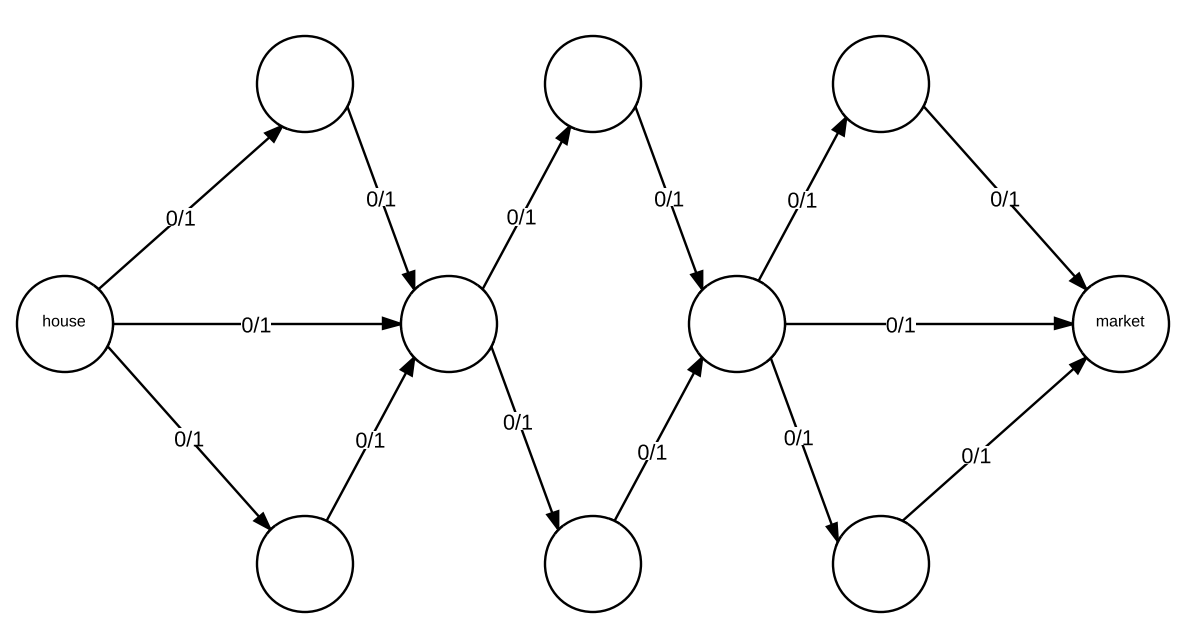
\includegraphics[scale=0.5]{./img/ps9-4.png}
        \caption{Example Graph}
    \end{figure}

    Once we have a graph, we can simply run our Ford-Fulkerson Algorithm in order to see possibilities. Below would be
    one possibility of our working example graph from above.

    \begin{figure}[H]
        \centering
        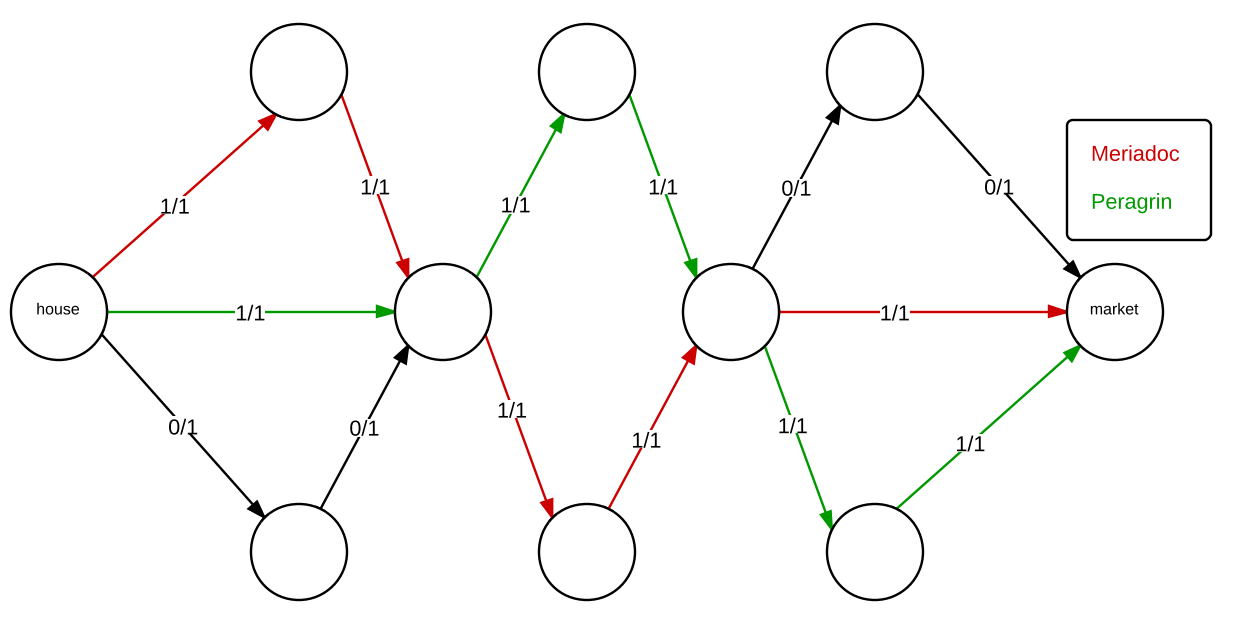
\includegraphics[scale=0.5]{./img/ps9-4-a.png}
        \caption{Example Graph after Ford-Fulkerson}
    \end{figure}

    @ Preparing for a big end-of-semester party in The Shire, you open your cellar and count $n$ bottles of fine wine.
    Gandalf has previously warned you that exactly $k$ of these bottles have been poisoned, and consuming poisoned wine
    will result in an unpleasant death. The party starts in one hour, and you do not want to poison any of your
    guests.\newline

    Luckily, a family of $l$ docile rats occupies a corner of the cellar, and they have graciously volunteered to be
    test subjects for identifying the poisoned bottles. Let $l = o(n)$ and $k = 1$, and assume it takes just under one
    hour for poisoned wine to kill a rat.  Describe a scheme by which you can feed wine to rats and identify with
    complete certainty the poisoned bottle, prove that the scheme is correct and give a tight bound on the number of
    rats $l$ necessary to solve the problem.

    @@ A naive approach is simply to feed $n$ rats a drop from each of the $n$ bottles. This results in requiring $n$
    rats. We can do better.\newline

    Number all of the bottles of wine $0, \ldots, n$. Number all of the rats $0, \ldots, l$. Now convert all of the wine
    bottle labels to binary, yielding a set of bottles with numbering $\left\{ 0, 1, 10, 11, 100, \ldots \right\}$. For
    each bottle, the bit indicates which rat we feed that bottle to. For instance, bottle $10110$ would be fed to rats
    1, 2, 4. When we do this the rats now act as ``bits''. After an hour if we look at which rats have died and
    reconstruct the bits from them, we'll get the label of the poisoned bottle.\newline

    For instance, let there be 10 bottles of wine. These are numbered as $0$ through $1001$, and we need 4 rats to
    determine the poison.

    \begin{table}[H]
        \centering
        \begin{tabular}{|l||l|l|l|l|}
            \hline
            \textit{Bottle Label} & 0 & 1 & 2 & 3\\
            \hline
            \hline
            0 & N & N & N & N\\
            1 & Y & N & N & N\\
            10 & N & Y & N & N\\
            11 & Y & Y & N & N\\
            100 & N & N & Y & N\\
            101 & Y & N & Y & N\\
            110 & N & Y & Y & N\\
            111 & Y & Y & Y & N\\
            1000 & N & N & N & Y\\
            1001 & Y & N & N & Y\\
            \hline
        \end{tabular}
        \caption{Wine and Rats}
    \end{table}

    We can see that if (for instance) rats 0 and 2 die, bottle 101 is poisoned.\newline

    This method requires $\log(n)$ rats since we're using bits, which is significantly better than $n$.
\end{easylist}
\end{document}
